% 一线三直角（K 字直角特例 α=90°）：中考最高频
% 由 △ACP ∼ △PBD 得 AC·BD = AP·PB；取 AP=PB=2、AC=1.5 → BD=4/1.5≈2.667
\documentclass[tikz,border=4pt]{standalone}
\usetikzlibrary{calc}
\begin{document}
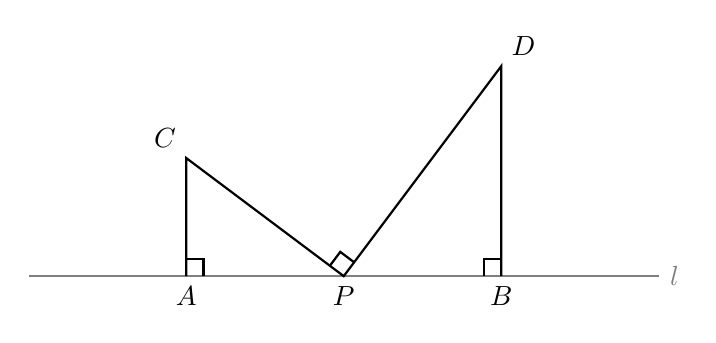
\begin{tikzpicture}[scale=1.0, thick]
  \draw[gray] (-4, 0) -- (4, 0);
  \node[gray] at (4.2, 0) {$l$};

  \coordinate (A) at (-2, 0);
  \coordinate (P) at (0, 0);
  \coordinate (B) at (2, 0);
  \coordinate (C) at (-2, 1.5);
  \coordinate (D) at (2, 2.667);

  \draw (A) -- (C) -- (P) -- (D) -- (B);

  % 三个直角符号
  % ∠CAP（A 点）
  \draw ($(A) + (0.22, 0)$) -- ($(A) + (0.22, 0.22)$) -- ($(A) + (0, 0.22)$);
  % ∠DBP（B 点）
  \draw ($(B) + (-0.22, 0)$) -- ($(B) + (-0.22, 0.22)$) -- ($(B) + (0, 0.22)$);
  % ∠CPD（P 点）：PC 方向 atan2(1.5,-2)≈143.13°、PD 方向 atan2(2.667,2)≈53.13°，差 90°
  % 直角符号沿这两方向各取 0.22 长度的两段
  \coordinate (pc) at ({0.22*cos(143.13)}, {0.22*sin(143.13)});
  \coordinate (pd) at ({0.22*cos(53.13)},  {0.22*sin(53.13)});
  \draw (pc) -- ($(pc) + (pd)$) -- (pd);

  \node[below] at (A) {$A$};
  \node[below] at (P) {$P$};
  \node[below] at (B) {$B$};
  \node[above left]  at (C) {$C$};
  \node[above right] at (D) {$D$};
\end{tikzpicture}
\end{document}
